
\newpage

%!TEX root = tro-ids.tex

\section{Application to Automated Transportation Systems in Urban Environment} 
\label{sec:example:highway}

In this section we describe the application of our technique to a first cooperative system, consisting of a group of $n$ cars moving along an $m$ lane highway (see Fig.~\ref{fig:car-neigh} for a depiction with $m=3$). The system can be formalized as an instance of the cooperation protocol~$\P$ presented in Section~\ref{sec:model}. Cars have their own dynamics $f_i$ and local controllers $u_i$, but their pilots are supposed to follow the European, right--hand traffic rules to avoid collisions. Every car $\ai$ is assigned a {\color{red} $v_{des, i}$, which is a constant state variable ($\dot{v_{des, i}} = 0$) indicating the speed at which each car desires to travel and is supposed to be measured as any other state variable.} Each car must decide on a suitable motion maneuver, i.e., accelerate ($\mfast$) or decelerate ($\mslow$), change to the next left lane ($\mleft$) or to the right one ($\mright$), based on the presence or absence of other cars in its neighborhood. E.g., the presence of a slower car in the
front, and a free lane on the left requires the execution of an
overtake that is a change from a $\mfast$ to a $\mleft$ maneuver. {\color{red} In addition to these four maneuvers, in this system we examine the possibility of a fifth one called $\mplatoon$, which defines a mode characterized by an oscillating longitudinal motion between the preceeding and/or following car.} The
rules require the introduction of a topology $\eta_{i,1}(q_i)$
representing a region in the immediate front of an agent~$\ai$ {\color{red} and longitudinal size $d_{f}$}, a
topology $\eta_{i,2}(q_i)$ for a region on its left {\color{red} and longitudinal size $d_f + d_b$}, a topology
$\eta_{i,3}(q_i)$ for a region on its right {\color{red} and longitudinal size $d_f + d_b$}, and a topology
$\eta_{i,4}(q_i)$ for a region on its back {\color{red} and longitudinal size $d_b$} (see again, Fig.~\ref{fig:car-neigh}), {\color{red}
a topology $\eta_{i,5}(q_i)$ for a region in front of it and longitudinal size $d_{int}$, $\eta_{i,6}(q_i)$ for a region on its back and longitudinal size $d_{int}$, where $d_f$ and $d_b$ are a forward and backward safety distances, $d_{int}$ is the interaction distance, smaller than the visible distance but larger than $d_f$ and $d_b$. We also define three more topologies $\eta_{i,7}(q_i)$, $\eta_{i,8}(q_i)$, $\eta_{i,9}(q_i)$ which are not simple areas in the highway plane, but also depend on another state variable ($v_{des}$). These topologies respectively describe the state-space area in front of the agent, on its back and on its right with compatible  $v_{des}$ (for the first two) and smaller $v_{des}$ (for the last one). The last one also intuitively refers to the state-space region of a car that can be overataken by~$\ai$. What we mean by `compatible' and `smaller' will be better expressed with the formal definition of the topologies. 
 }
%%
\begin{figure}
\centering
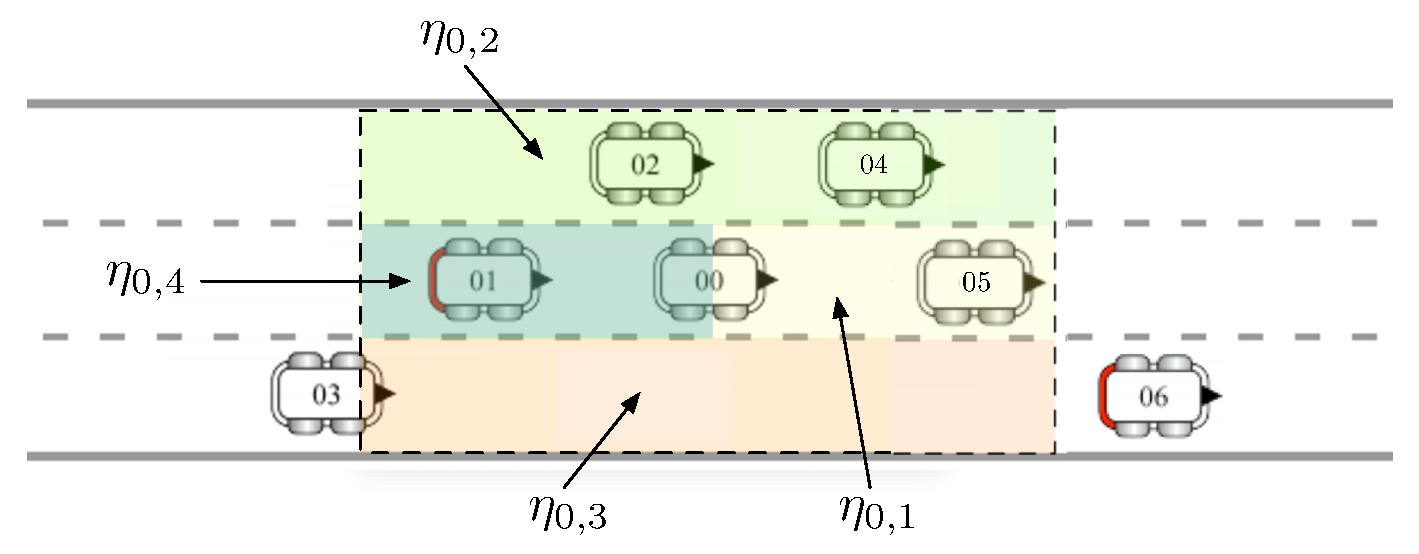
\includegraphics[width=0.45\textwidth,clip]{images/highway-topology.pdf}\\
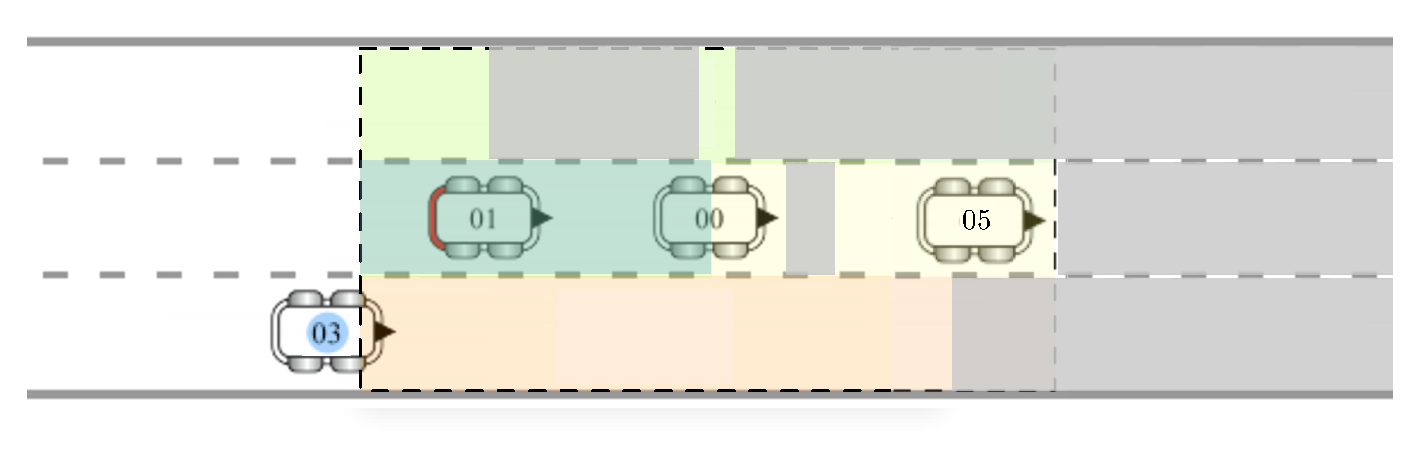
\includegraphics[width=0.45\textwidth,clip]{images/highway-visibility.pdf}\\
\caption{Neighborhood topologies of an agent (above) and partial visibility of a local monitor (below) in the highway example. {\color{red} For clarity's sake, only the first four topologies are shown in this picture.}}
\label{fig:car-neigh}
\end{figure}
%%
%Note that these rules apply to very large systems with an unbounded number of vehicles, yet they only require that every car verifies the existence and/or absence of $N$ other cars in its vicinity, where $N$ is a small number depending only on the geometry of the lanes and of the vehicles.

%A complete description of the system's formalization is reported in Appendix~\ref{sec:highway}. 
%%
%\begin{figure*}[!]
%\centering
%\fbox{%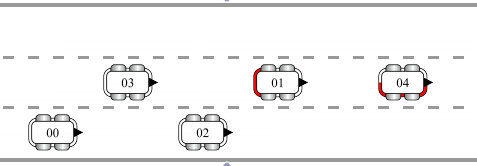
\includegraphics[width=0.64\columnwidth,clip]{images/highway-1.png}}
%\vspace{5pt}
%\fbox{%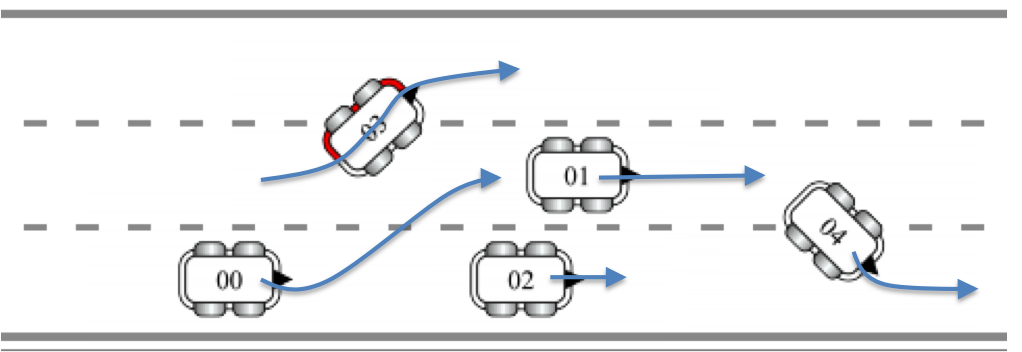
\includegraphics[width=0.64\columnwidth,clip]{images/highway-2-arrow.png}}
%\vspace{5pt}
%\fbox{%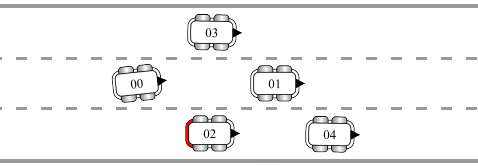
\includegraphics[width=0.64\columnwidth,clip]{images/highway-3.png}}\\
%\caption{Example of cooperative system where agents are cars in a highway that are supposed to follow the common driving rules to avoid collisions. 
%%Car $01$ initially slows down for the presence on its front lane of car $04$, that in turn turns right as its next right lane is free. Car $03$ later starts a left turn as car $01$ occupies its immediate front lane and its next left lane is free. Finally, car $02$ slows down as its front lane is occupied by car $04$ and its next left lane is also occupied by the cars $00$ and $01$.
%} 
%\label{fig:highway-simulation}
%\end{figure*}
%%%%

%Consider $n$ cars that are supposed to follow the European, right--hand traffic rules while traveling along a highway with $m$ lanes. Every car $\ai$ must coordinate its motion with neighboring cars as follows: accelerate up to its allowed maximum speed $v_{max}^i$ if the current lane is free; change to the next left lane if the current one is occupied by a preceding car and there are no cars on the immediate back; reduce speed and remain in the current lane otherwise; try to proceed along the next right lane when possible; do not overtake on the right.

%Referring to Fig.~\ref{fig:car-config}, the configuration of a generic car $\ai$ is $q_i =  (x_i, y_i, \theta_i, v_i)$, where $(x_i,y_i)$ is the position of the car's center, $\theta_i$ is its orientation w.r.t. the $x$--axis, and $v_i$ is its forward speed. 
%%
%\begin{figure}
%\centering
%%\includegraphics[width=0.6\columnwidth,clip]{images/ids/model/car-config.pdf}
%\caption{Mechanical configuration of a generic car $\mathcal{A}_i$.}
%\label{fig:car-config}
%\end{figure}
%%

The system can be described as an instance of $\mathcal{P}$ with the environment, the configuration $q_i$ and the dynamic map $f_i : \Q \times \Sigma_i \rightarrow T_\Q$ described in Section~\ref{sec:model}. The above introduced topologies can be formalized as follows:
\begin{equation*}
\begin{array}{rcl}
\eta_{i,1} := \eta_{i, forwardBlock} & : & \Q \rightarrow 2^\Q \\
& & q_i \mapsto \left\lbrace (x,y,\theta, v, v_{des}) \, | \, x_i \leq x \leq x_i + d_f, \right. \\ & & \;\;\;\;\;\;\;\;\;\;\;\;\;\;\;\;\;\;\;\; \left. \lfloor \frac{y_i}{w} \rfloor w \leq y \leq \left( \lfloor \frac{y_i}{w} \rfloor + 1 \right) w \right\rbrace \, , \\
%
\eta_{i,2} := \eta_{i, leftBlock} & : & \Q \rightarrow 2^\Q \\
& & q_i \mapsto \left\lbrace (x,y,\theta, v, v_{des}) \, | \, x_i-d_b \leq x \leq x_i + d_f, \right. \\ & & \;\;\;\;\;\;\;\;\;\;\;\;\;\;\;\;\;\;\;\; \left. \left( \lfloor \frac{y_i}{w} \rfloor + 1 \right) w \leq y \leq \left( \lfloor \frac{y_i}{w} \rfloor + 2 \right) w \right\rbrace \, , \\
%
\eta_{i,3} := \eta_{i, rightBlock} & : & \Q \rightarrow 2^\Q \\
& & q_i \mapsto \left\lbrace (x,y,\theta, v, v_{des}) \, | \, x_i-d_b \leq x \leq x_i + d_f, \right. \\ & & \;\;\;\;\;\;\;\;\;\;\;\;\;\;\;\;\;\;\;\; \left. \left( \lfloor \frac{y_i}{w} \rfloor - 1 \right) \leq y \leq \lfloor \frac{y_i}{w} \rfloor w \right\rbrace \, , \\
%
\eta_{i,4} := \eta_{i, backBlock} & : & \Q \rightarrow 2^\Q \\
& & q_i \mapsto \left\lbrace (x,y,\theta, v, v_{des}) \, | \, x_i-d_b \leq x \leq x_i, \right. \\ & & \;\;\;\;\;\;\;\;\;\;\;\;\;\;\;\;\;\;\;\; \left. \lfloor \frac{y_i}{w} \rfloor w \leq y \leq \left( \lfloor \frac{y_i}{w} \rfloor + 1 \right) w \right\rbrace \, , \\
%
\eta_{i,5} := \eta_{i, forwardPresent} & : & \Q \rightarrow 2^\Q \\
& & q_i \mapsto \left\lbrace (x,y,\theta, v, v_{des}) \, | \, x_i \leq x \leq x_i +d_{int}, \right. \\ & & \;\;\;\;\;\;\;\;\;\;\;\;\;\;\;\;\;\;\;\; \left. \lfloor \frac{y_i}{w} \rfloor w \leq y \leq \left( \lfloor \frac{y_i}{w} \rfloor + 1 \right) w \right\rbrace \, , \\
%
\eta_{i,6} := \eta_{i, backPresent} & : & \Q \rightarrow 2^\Q \\
& & q_i \mapsto \left\lbrace (x,y,\theta, v, v_{des}) \, | \, x_i-d_{int} \leq x \leq x_i, \right. \\ & & \;\;\;\;\;\;\;\;\;\;\;\;\;\;\;\;\;\;\;\; \left. \lfloor \frac{y_i}{w} \rfloor w \leq y \leq \left( \lfloor \frac{y_i}{w} \rfloor + 1 \right) w \right\rbrace \, , \\
%
\eta_{i,7} := \eta_{i, forwardCompatible} & : & \Q \rightarrow 2^\Q \\
& & q_i \mapsto \left\lbrace (x,y,\theta, v, v_{des}) \, | \, x_i \leq x \leq x_i + d_{int}, \right. \\ 
 & & \;\;\;\;\;\;\;\;\;\;\;\;\;\;\;\;\;\;\;\; 
\left. \lfloor \frac{y_i}{w} \rfloor w \leq y \leq \left( \lfloor \frac{y_i}{w} \rfloor + 1 \right) w \right. \\ 
& & \;\;\;\;\;\;\;\;\;\;\;\;\;\;\;\;\;\;\;\;
\left. (1 - f)v_{des, i} \leq v_{des} \leq (1+f)v_{des, i} \right.
\rbrace \, , \\
%
\eta_{i,8} := \eta_{i, backCompatible} & : & \Q \rightarrow 2^\Q \\
& & q_i \mapsto \left\lbrace (x,y,\theta, v, v_{des}) \, | \, x_i - d_{int}\leq x \leq x_i, \right. \\ 
 & & \;\;\;\;\;\;\;\;\;\;\;\;\;\;\;\;\;\;\;\; 
\left. \lfloor \frac{y_i}{w} \rfloor w \leq y \leq \left( \lfloor \frac{y_i}{w} \rfloor + 1 \right) w \right. \\ 
& & \;\;\;\;\;\;\;\;\;\;\;\;\;\;\;\;\;\;\;\;
\left. (1 - f)v_{des, i} \leq v_{des} \leq (1+f)v_{des, i} \right.
\rbrace \, , \\
%
\eta_{i,9} := \eta_{i, rightOvertakeable} & : & \Q \rightarrow 2^\Q \\
& & q_i \mapsto \left\lbrace (x,y,\theta, v, v_{des}) \, | \, x_i - d_{int}\leq x \leq x_i, \right. \\ 
 & & \;\;\;\;\;\;\;\;\;\;\;\;\;\;\;\;\;\;\;\; 
\left. \left( \lfloor \frac{y_i}{w} \rfloor - 1 \right) \leq y \leq \lfloor \frac{y_i}{w} \rfloor w \right. \\ 
& & \;\;\;\;\;\;\;\;\;\;\;\;\;\;\;\;\;\;\;\;
\left. v_{des} \leq (1-f)v_{des, i} \right.
\rbrace \,  \\

 
 
\end{array}
\end{equation*}
where $w$ is the lane width, {\color{red}$f$ is a constant indicating the relative tolerance in $v_{des}$} and $\lfloor \cdot \rfloor$ returns the nearest lower integer of the argument. Thus, the encoder map is $s_i :  \Q \times \Q^{n_i} \rightarrow \bool^9$, $s_i = (s_{i,1}, \cdots, s_{i,9})$, and the agent's neighborhood is $N(q_i) = \eta_{i,1}(q_i) \cup \cdots \cup \eta_{i,9}(q_i)$. Moreover, we need to introduce two constants $\lambda_{i,1}, \lambda_{i,2}$ representing the left--most and right--most lanes, respectively, and two constants $\lambda_{i,3}, \lambda_{i,4}$ representing the current target lane's left and right edges, respectively. Finally, 
we define a $\lambda_{i, 5}$ indicating if the agent is lined up with its lane:
\begin{equation*}
\begin{array}{rcl}
\lambda_{i,1} := \lambda_{i, minLane} & = & \left\lbrace (x,y,\theta, v, v_{des}) \, | \, (m-1) w \leq y \leq m \, w \right\rbrace \, , \\
%
\lambda_{i,2} := \lambda_{i, maxLane} & = & \left\lbrace (x,y,\theta, v, v_{des}) \, | \, 0 \leq y \leq w \right\rbrace \, , \\
%
\lambda_{i,3} := \lambda_{i, targetLeftLane} & = & \left\lbrace (x,y,\theta, v, v_{des}) \, | \, y \geq \left( \left\lfloor \frac{y_i(t_k)}{w} \right\rfloor + 1 \right) w \right\rbrace \, , \\
%
\lambda_{i,4} := \lambda_{i, targetRightLane} & = & \left\lbrace (x,y,\theta, v, v_{des}) \, | \, y \leq \left( \left\lfloor \frac{y_i(t_k)}{w} \right\rfloor \right) w \right\rbrace \, , \\
%
\lambda_{i,5} := \lambda_{i, linedUp} & = & \left\lbrace (x,y,\theta, v, v_{des}) \, | \, |y - \lfloor \frac{y}{w} \rfloor w - \frac{w}{2} | \leq \Delta_y \right. \, , \\ 
& & \;\;\;\;\;\;\;\;\;\;\;\;\;\;\;\;\;\;\;\;\;\;\;\;\;\; 
|\theta| \leq \Delta_{\theta}  \rbrace \\

\end{array}
\end{equation*}

{\color{red}where $\Delta_x$ are constant tolerances of the variable $x$, and $t_k$ is the instant at which an event was detected. Through these constants we
define the constant map $r_i :  \Q \rightarrow \bool^5$, $r_i = (r_{i,1}, \cdots, r_{i,5})$.}
The event alphabet is $E_i = \{e^{i,1}, \cdots, e^{i,21}\}$ and the detector map $e_i \in \bool \rightarrow 2^{E_i}$ is characterized by the event conditions 
\begin{equation*}
\begin{array}{l}
%%% FAST -> SLOW
c_{i,1} = s_{i,1} \, s_{i,2} \, \neg s_{i, 7} \, r_{i, 5}\, , \;\;
c_{i,2} = s_{i, 1} \, \neg s_{i, 7} \, r_{i, 2} \, r_{i, 5} \, , \;\;
c_{i,3} = s_{i,1} \, \neg s_{i,7} \, \neg r_{i, 5} \, , \;\; 
c_{i,4} = \neg s_{i,1} \, s_{i,3} \, s_{i, 7} \, \neg s_{i, 9} \, , \;\;
\\
%%% FAST -> LEFT
c_{i,5} = s_{i,1} \, \neg s_{i, 2} \, \neg s_{i, 7} \, \neg r_{i, 2} \, r_{i, 5}\, , \;\;
\\
%%% FAST -> RIGHT
c_{i,6} = \neg s_{i,1} \, \neg s_{i, 3} \, \neg r_{i, 1} \, r_{i, 5} \, , \;\;
\\
%%% SLOW -> FAST
c_{i,7} = \neg s_{i,1} \, s_{i, 9}, \;\;
c_{i,8} = \neg s_{i, 1} \, \neg s_{i, 3} \, , \;\;
\\
%%% SLOW -> LEFT
c_{i,9} = s_{i, 1} \, \neg s_{i, 2} \, \neg r_{i, 2} \, r_{i,5} \, , \;\;
\\
%%% LEFT -> FAST
c_{i,10} = \neg s_{i,7} \, r_{i,3} \, , \;\;
\\
%%% RIGHT -> FAST
c_{i,11} = \neg s_{i,7} \, r_{i,4} \, , \;\;
\\
%%% PLATOON -> FAST
c_{i,12} =  \neg s_{i, 7} \, \neg s_{i, 8} , \;\;
c_{i,13} =  \neg s_{i, 3} \, \neg s_{i, 5} \, s_{i, 6} \, r_{i, 1}, \;\;
\\
%%% PLATOON -> SLOW
c_{i,14} =  \neg s_{i, 1} \,  s_{i, 3} \, \neg s_{i, 9}\;\;
\\
%%% PLATOON -> LEFT
c_{i, 15} = s_{i, 1} \, \neg s_{i, 2} \, \neg s_{i, 7} \, \neg r_{i, 2} \;\;
\\
%%% FAST -> PLATOON
c_{i, 16} = s_{i, 7} \;\;
c_{i, 17} = s_{i, 3} \, s_{i, 8} \;\;
c_{i, 18} = s_{i, 1} \, s_{i, 2} \, \neg s_{i, 7} \, s_{i, 8}
c_{i, 19} = s_{i, 1} \, \neg s_{i, 7} \, s_{i, 8}, r_{i, 2} \;\;
\\
%%% LEFT -> PLATOON
c_{i, 20} = s_{i, 7} \, r_{i, 3} \;\;
\\
%%% RIGHT -> PLATOON 
c_{i, 21} = s_{i, 7} \, r_{i, 4}
\\
\end{array}
\end{equation*}
The finite set of discrete states is $\Sigma_i=\{\mfast, \mslow,$ $\mleft, \mright,  \mplatoon\}$ ($p=5$) and the automaton's dynamics is 
\begin{equation*}
\begin{array}{rcl}
%%% FAST -> FAST
\delta_i & : & \Sigma_i \times 2^{E_i} \rightarrow \Sigma_i  \\
& & \begin{array}{l} \left((\mfast, \neg (e^{i,1} + e^{i, 2} + e^{i, 3} + e^{i, 4} + e^{i,5}
+ e^{i, 6} + e^{i, 16} + e^{i, 17} + e^{i, 18} + e^{i, 19})\right) \end{array} \mapsto \mfast \, , \\
%%% FAST -> SLOW
& & \begin{array}{l} (\mfast, e^{i,1}), (\mfast, e^{i,2}), (\mfast, e^{i,3}), (\mfast, e^{i,4}) \end{array} \mapsto \mslow \, , \\
%%% FAST -> LEFT
& & \begin{array}{l} (\mfast, e^{i,5}) \end{array} \mapsto \mleft, \\
%%% FAST -> RIGHT
& & \begin{array}{l} (\mfast, e^{i,6}) \end{array} \mapsto \mright, \\
%%% FAST -> PLATOON
& & \begin{array}{l} (\mfast, e^{i,16}), (\mfast, e^{i,17}), (\mfast, e^{i,18}), (\mfast, e^{i, 19}) \end{array} \mapsto \mplatoon, \\
%%% SLOW -> SLOW
& & \begin{array}{l} \left((\mslow, \neg (e^{i,7} + e^{i, 8} + e^{i, 9})\right) \end{array} \mapsto \mslow \, , \\
%%% SLOW -> FAST
& & \begin{array}{l} (\mslow, e^{i,7}), (\mslow, e^{i,8}) \end{array} \mapsto \mfast 
\\
%%% SLOW -> LEFT
& & \begin{array}{l} (\mslow, e^{i,9})) \end{array} \mapsto \mleft 
\\
%%% LEFT -> LEFT
& & \begin{array}{l} \left((\mleft, \neg (e^{i,10} + e^{i, 20})\right) \end{array} \mapsto \mleft \, , \\
%%% LEFT -> FAST
& & \begin{array}{l} (\mleft, e^{i,10})) \end{array} \mapsto \mfast 
\\
%%% LEFT -> PLATOON
& & \begin{array}{l} (\mleft, e^{i,20})) \end{array} \mapsto \mplatoon 
\\
%%% RIGHT -> RIGHT
& & \begin{array}{l} \left((\mright, \neg (e^{i,11} + e^{i, 21})\right) \end{array} \mapsto \mright \, , \\
%%% RIGHT -> FAST
& & \begin{array}{l} (\mright, e^{i,11})) \end{array} \mapsto \mfast 
\\
%%% RIGHT -> PLATOON
& & \begin{array}{l} (\mright, e^{i,21})) \end{array} \mapsto \mplatoon 
\\
%%% PLATOON -> PLATOON
& & \begin{array}{l} \left((\mplatoon, \neg (e^{i,12} + e^{i, 13} + e^{i, 14} + e^{i, 15})\right) \end{array} \mapsto \mplatoon \, , \\
%%% PLATOON -> FAST
& & \begin{array}{l} (\mplatoon, e^{i,12})), (\mplatoon, e^{i,13})) \end{array} \mapsto \mfast \\
%%% PLATOON -> SLOW
& & \begin{array}{l} (\mplatoon, e^{i,14})) \end{array} \mapsto \mslow \\
%%% PLATOON -> LEFT
& & \begin{array}{l} (\mplatoon, e^{i,15})) \end{array} \mapsto \mleft \\

\end{array}
\end{equation*}
with initial state $\sigma_i^0 = \mfast$.
%%
%\begin{figure}
%\centering
%%\includegraphics[width=0.8 \columnwidth,clip]{images/ids/model/car-automaton.pdf}
%\caption{Dynamics $\delta$ of the cooperation manager for an autonomous car.}
%\label{fig:car-manager}
%\end{figure}
%%

The decoder map is $u_i :  \Q \times \Sigma_i \rightarrow \U_i$, $u_i = (a_i, \omega_i)$, with
\begin{equation*}
\begin{array}{rcl}
a_i  & : & \Q \times \Sigma_i \rightarrow \real \\
& & \begin{array}{l} (q_i, \mfast), (q_i, \mleft), \\ (q_i, \mright) \end{array}
\mapsto 
\left \lbrace
\begin{array}{cl}
\bar{a} & \mathrm{if} \ v_i < v_{des, i} \\
0 & \mathrm{otherwise}
\end{array}
\right. \, ,
\\
& & \begin{array}{l} (q_i, \mslow) \end{array} 
\mapsto 
\left \lbrace
\begin{array}{cl}
-\bar{a} & \mathrm{if} \ v_i > 0 \\
0 & \mathrm{otherwise}
\end{array}
\right. \, , \\
& & \begin{array}{l} (q_i, \mplatoon) \end{array} 
\mapsto 
\left \lbrace
\begin{array}{cl}
-b_b(x_i - x_{b}) - b_f(x_i - x_f) - \gamma b_b (v_i - v_b) - \gamma b_f (v_i - v_f) & \mathrm{if} \textcircled{1}\\
-b_f(x_i - x_{f} + d_{ref}) - \gamma b_f(v_i - v_f) & \mathrm{if} \textcircled{2} \\
-b_b(x_i - x_{b} - d_{ref}) - \gamma b_b k_{leader} (v_i - v_{des}) & \mathrm{if} \textcircled{3} \\
-b_b(x_i - x_{b} - d_{ref}) - b_f(x_i - x_f + d_f) - \gamma b_b (v_i - v_b) - \gamma b_f (v_i - v_f) & \mathrm{if} \textcircled{4} \\
 \end{array}
\right. \, ,
\end{array}
\end{equation*}
\begin{equation*}
\begin{array}{rcl}
\omega_i  & : & \Q \times \Sigma_i \rightarrow \real \\
& & \begin{array}{l} (q_i, \mfast), \\ (q_i, \mslow) \\ (q_i, \mplatoon) \end{array}
\mapsto 
\left( \left( y^*(q_i) - y_i \right) \frac{\sin\theta_i}{\theta_i} - \mu \, \theta_i \right) v_i \, , \\
& &  \begin{array}{l}  (q_i, \mleft), \end{array} \mapsto 
\left \lbrace
\begin{array}{cl}
\bar{\omega} & \mathrm{if} \ \theta_i < \theta_{max} \\
0 & \mathrm{otherwise}
\end{array}
\right. \, , 
\\
& &  \begin{array}{l} (q_i, \mright)  \end{array} \mapsto 
\left \lbrace
\begin{array}{cl}
-\bar{\omega} & \mathrm{if} \ \theta_i > - \theta_{max} \\
0 & \mathrm{otherwise}
\end{array}
\right. \, ,
\end{array} 
\end{equation*}
{\color{red} where $b_b$, $b_f$, $\gamma$, $k_{leader}$ are positive constants, $d_f$ is the aforementioned forward safety distance}, $y^*(q_i) = \left( \left\lfloor \frac{y_i}{w} \right\rfloor + \frac{1}{2} \right) w$ is the current lane center, $\theta_{max}$ is the agent's maximum curvature angle, and $\mu$, $\bar{a}$ and $\bar{\omega}$ are positive constants {\color{red}and the conditions are defined as follows:}
\begin{equation*}
\begin{array}{cl}
\left \lbrace 
\begin{array}{l}
\textcircled{1}: \mathsf{Vehicles \, in \, front \, of \, and \, behind~\ai \, have \, compatible \, v_{des}\,} \\
\textcircled{2}: \mathsf{Only \, the \, vehicle \, in \, front \, of ~\ai \, have \, a compatible \, v_{des}\,}\\
\textcircled{3}: \mathsf{The \, vehicle \, behind~\ai \, has \, a \, compatible \, v_{des}\, and \, no \, vehicles \, are \, blocking \, the \, forward \, area}\\
\textcircled{4}: \mathsf{The \, vehicle \, behind~\ai \, has \, a \, compatible \, v_{des}\, and \, a \, vehicle \, is \, blocking \, the \, forward \, area}
\end{array}
\right.
\end{array}
\end{equation*}

{\color{red}These conditions respectively describe the controller of a vehicle in the middle of a platoon, in the tail, the platoon leader and a forced platoon situation that arises when the agent cannot overtake a slower vehicle.}\\

Finally, the visibility map returns the set of configurations laying within a distance $R_i$ and that are not hidden by other cars (see e.g. the known sweeping line algorithm in~\cite{thrun2002pr} for its computation, and the examples in Fig.~\ref{fig:ids:model:visi}). A formal description of the map is avoided for space reasons.
%%
\begin{figure*}[!]
\centering
\fbox{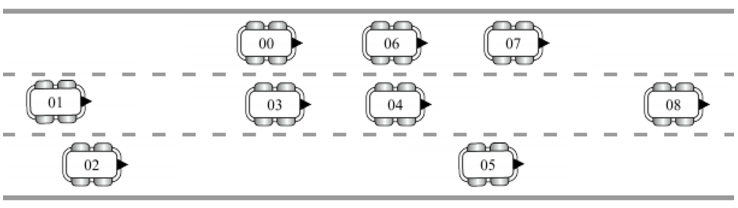
\includegraphics[width=0.32\textwidth,clip]{images/example_01.pdf}}
\\
\vspace{5pt}
\fbox{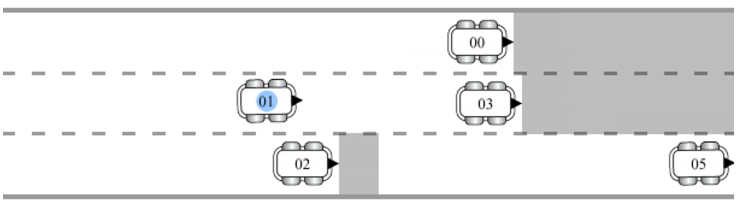
\includegraphics[width=0.32\textwidth,clip]{images/example_01_a.pdf}}
\vspace{5pt}
\fbox{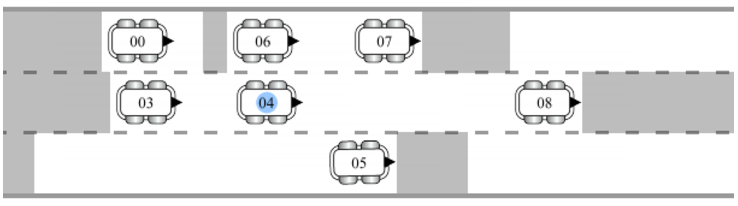
\includegraphics[width=0.32\textwidth,clip]{images/example_01_b.pdf}}
\\
\caption{Sensing model in the highway example: from left to right, complete state of the system and views of agents $\mathcal{A}_1$ and $\mathcal{A}_4$, respectively.}
\label{fig:ids:model:visi}
\end{figure*}


\subsection{Local Monitors}

Consider four cars in the highway example (Fig.~\ref{fig:highway_faulty_a}--a). Misbehavior of car~$0$, running a $\mfast$ maneuver along the second lane, while its next right lane is free, has to be detected (the car should start a $\mright$ maneuver to return to the first lane). A $\mfast$ maneuver of a car in the second lane implies that the region on its right is occupied by another car. Three local monitors on the other cars try to learn whether the car~$0$ is cooperative or not, but have only partial view of the car's neighborhood. By means of the proposed local monitor, the three agents are able to compute estimates, $\hat{I}_{0}^{1}$, $\hat{I}_{0}^{2}$, and $\hat{I}_{0}^{3}$, of the occupancy map of car~$0$'s neighborhood, which are reported in Fig.~\ref{fig:highway_faulty_a}--b). However, the figure shows that all monitors are still unable to decide on the cooperativeness of the car~$0$, since there exist possible behaviors that comply with the cooperative model and their partial visibility.
%%
\begin{figure}
\centering
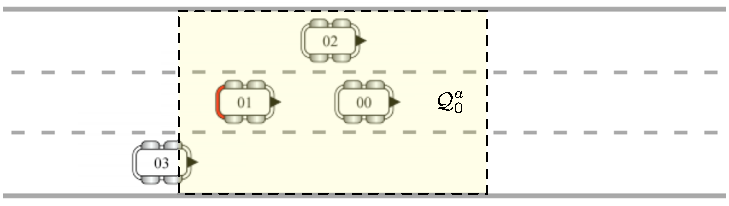
\includegraphics[width=0.47\textwidth]{images/simulation_01_F_a.pdf} \\
(a) \\
 \vspace{2mm}
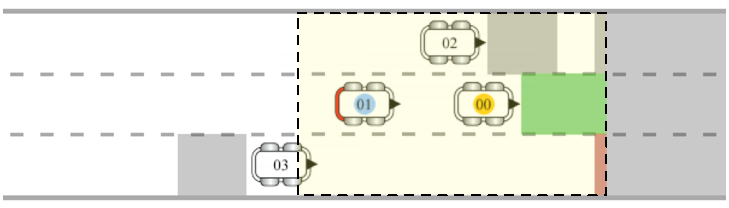
\includegraphics[width=0.47\textwidth]{images/simulation_01_A01_a.pdf} \\
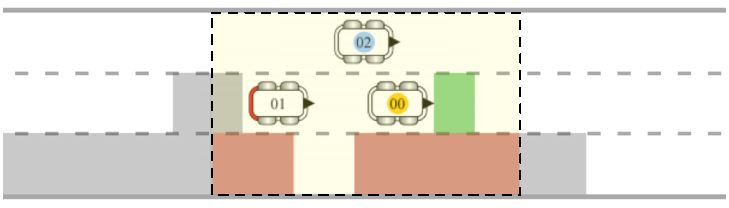
\includegraphics[width=0.47\textwidth]{images/simulation_01_A02_a.pdf} \\
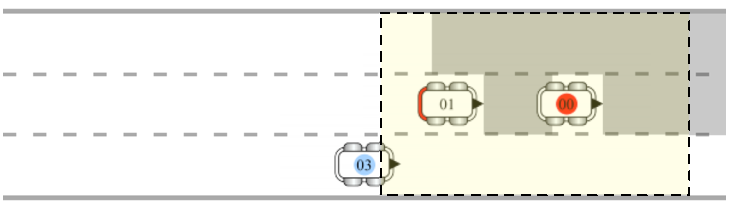
\includegraphics[width=0.47\textwidth]{images/simulation_01_A03_a.pdf} \\
(b)
\caption{Misbehavior of car~$0$, running a $\mfast$ maneuver along the second lane, while its next right lane is free, has to be detected (a). Local maps of occupancy, $\hat{I}_{0}^{1}$, $\hat{I}_{0}^{2}$, and $\hat{I}_{0}^{3}$, which local monitors on the cars $1$, $2$, and $3$ have reconstructed (b). The yellowish area dashed box outlines the target agent neighborhood; a blue circle specifies the current monitor; red (green) areas are non--visible regions, where the presence (absence) of a car is required. A colored circle around the target robot (green, yellow, or red) specifies its estimated cooperativeness ($\cooperative$, $\uncertain$, or $\uncooperative$, respectively).}
\label{fig:highway_faulty_a}
\end{figure}
%%

As a second example, consider eight cooperative cars in the highway and focus on the local view of car~$0$'s monitor (Fig.~\ref{fig:highway_2}). The presence of car~$07$ is detected (region $a$), based on the fact that car~$06$ is executing a $\mslow$ maneuver. The presence of car~$5$ is detected (regions $e$, and $f$), based on the $\mfast$ maneuvers on the second lane executed by cars $3$ and $4$. This also allows the detection of car absence in front of car~$3$ (region $b$) and car~$4$ (region $c$). To the local monitor all these neighboring cars are $\uncertain$, except car~$1$ that is certainly $\cooperative$. The example is used to show the fact that --- although this goes beyond the scope of the paper --- a local monitor's uncertainty in the classification of a neighbor can be reduced by cross--correlating maps of occupancies of different neighbors: the occupancy map $\hat{I}_{3}^{0}$ contains a free region ($b$ in the figure) in front of car~$3$, and an occupied region (the union of $d$ with $e$) on its right, while $\hat{I}_{2}^{0}$ contains a free region (same $d$ in the figure) in front of it. Therefore the region $d$ in $\hat{I}_{3}^{0}$ must be removed and the only possibly occupied region must be~$(e)$.
%%
\begin{figure}[!]
\centering
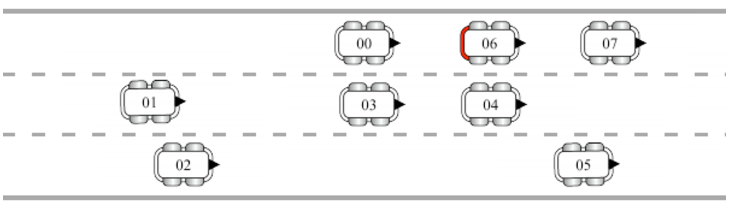
\includegraphics[width=0.47\textwidth]{images/simulation_02_F.pdf} \\
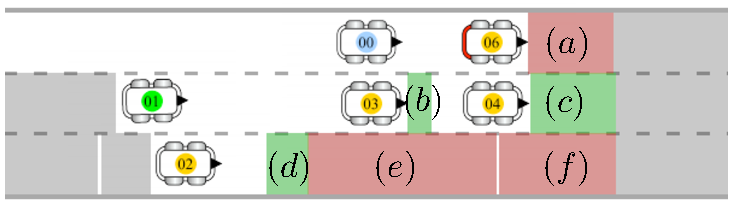
\includegraphics[width=0.47\textwidth]{images/monitor-everybody.pdf} \\
\caption{Eight cooperative cars (above) and view of the monitor on car~$00$ (below). A local monitor's uncertainty in the classification of a neighbor can be reduced by cross--correlating maps of occupancies of different neighbors.}
\label{fig:highway_2}
\end{figure}
%%

\subsection{Monitor Agreement via Set--valued Consensus}

%Theorem~\ref{th:consensus} provides us with sufficient conditions to realize a distributed iterative rule by which all local monitors can reach an agreement on the topology set of an agent~$\ai$. In particular, agents can start with initial estimates given by the locally estimated occupancy maps, i.e.,
%$$
%U_h = \hat{I}_i^h(t_k|t_{k+})
%$$
%and they can use the following merging function
%\begin{equation*}
%\begin{array}{rcl}
%\cap^* & : & 2^\Q  \times 2^\Q  \rightarrow 2^\Q  \\
%& & (X_1, X_2) \mapsto \{ x \, | \, \exists \, x_1 \in X_1 \setminus \emptyset, x_2 \in X_2 \setminus \emptyset \, | \, \\
%& & \;\;\;\;\;\;\;\;\;\;\;\;\;\;\;\;\;\;\;\;\;\;\;\; x = x_1 \cap x_2 \}
%\, .
%\end{array}
%\end{equation*}
%where $\cap$ is the set--theoretic intersection, which satisfies the theorem's hypotheses.

%$X_1 \sim X_2$ if, and only if, given $Z=F(X_1, X_2)$, $x \cap Z = \emptyset$ for all $x \in X_1 \cup X_2$

Consider the example in Fig.~\ref{fig:faulty-centr-example} where four cars~(2, 3, 4, and 5) are trying to reach a consensus on the misbehavior of a car (1 in the figure) remaining in the second lane. The cars can share their own local estimates of the occupancy map of car~$1$'s neighborhood, by sending one--hop (immediate neighbor) messages through a communication network described by a connected graph $G=(V_G,E_G)$, with $V_G = \{ 2, 3, 4, 5 \}$ and $E_G = \{e_{2,2}, e_{2,3}, e_{2,5}, e_{3,3}, e_{3,4}, e_{4,4},e_{5,5}\}$ (note that $\diam(G)=3$). The corresponding set--valued consensus protocol specializes to the following dynamic system:
%%
\begin{figure}[t!]
\centering
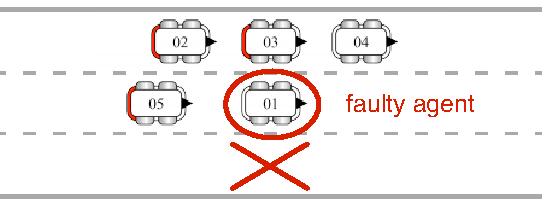
\includegraphics[width=0.38\textwidth,clip]{images/frame-b.pdf}
\caption{The misbehaving car~$1$ is executing a $\mfast$ maneuver on the second lane, while its next right lane is free.}
\label{fig:faulty-centr-example}
\end{figure}
%%
\begin{equation*}
\left\lbrace
\begin{array}{l}
X_2(k+1) = F^{(3)}(X_2(k), X_3(k), X_5(k)) =  \\
\;\;\;\;\;\;\;\;\;\;\;\;\;\;\;\;\, = X_2(k) \, \cap^* \, X_3(k) \, \cap^* \, X_5(k) \, , \\
X_3(k+1) = F^{(3)}(X_2(k), X_3(k), X_4(k)) =  \\
\;\;\;\;\;\;\;\;\;\;\;\;\;\;\;\;\, = X_2(k) \, \cap^* \, X_3(k) \, \cap^* \, X_4(k) \, , \\
X_4(k+1) =  F^{(2)}(X_3(k), X_4(k)) = X_3(k) \, \cap^* \, X_4(k) \, , \\
X_5(k+1) =  F^{(2)}(X_2(k), X_5(k)) =  X_2(k) \, \cap^* \, X_5(k) \, .
\end{array}
\right.
\end{equation*}
The system's evolution is reported in Fig.~\ref{fig:faulty-centr-consensus2}, where the $i$--th row represents the evolution of $X_i(t)$ (from left to right). No single local monitor has initially detected the misbehavior, which is instead iteratively obtained by car~$2$ and $3$ after two consensus steps and then by the other two cars. As expected from theory, all local monitors consent to the centralized estimated occupancy map (last column in the figure) 
$$
X^* = \hat{I}_1 = F^{(4)}(\hat{I}_1^2, \hat{I}_1^3, \hat{I}_1^4, \hat{I}_1^5)
$$
after at most $3$ steps.
%%
\begin{figure*}[!]
\centering
\begin{tabular}{ccccccc}
($k=0$) & ($k=1$) & ($k=2$) & ($k=3$) \\
\hspace{10pt}
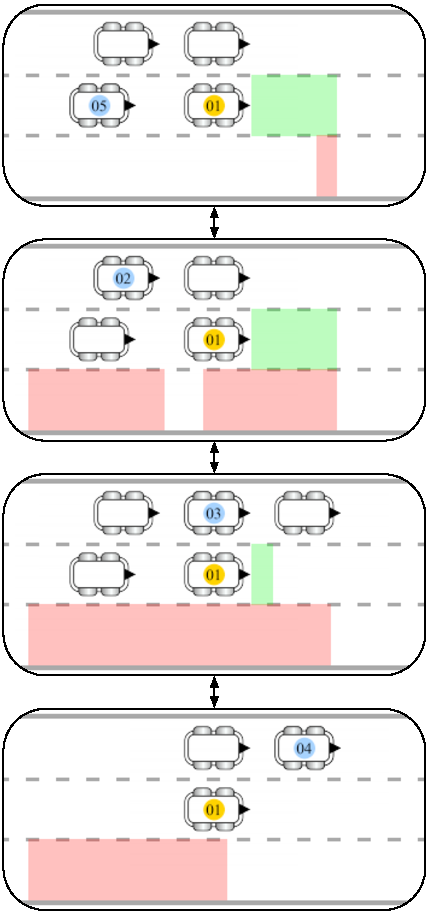
\includegraphics[width=0.22\textwidth,clip]{images/consensus-0.pdf}
&
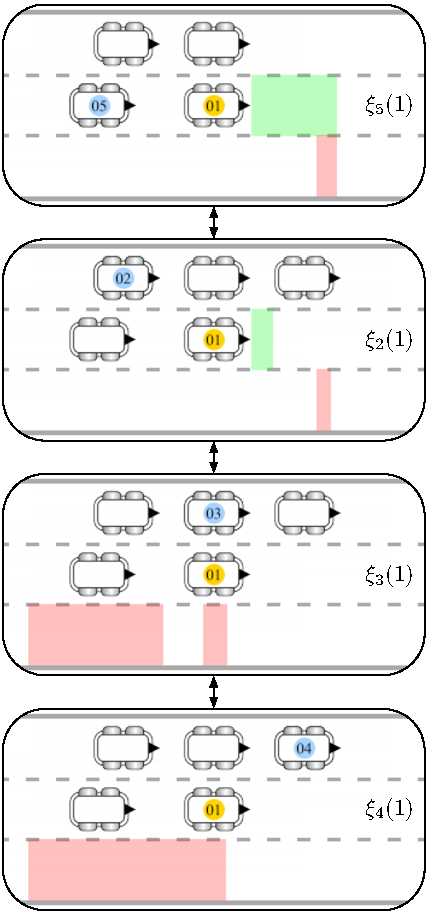
\includegraphics[width=0.22\textwidth,clip]{images/consensus-1.pdf}
&
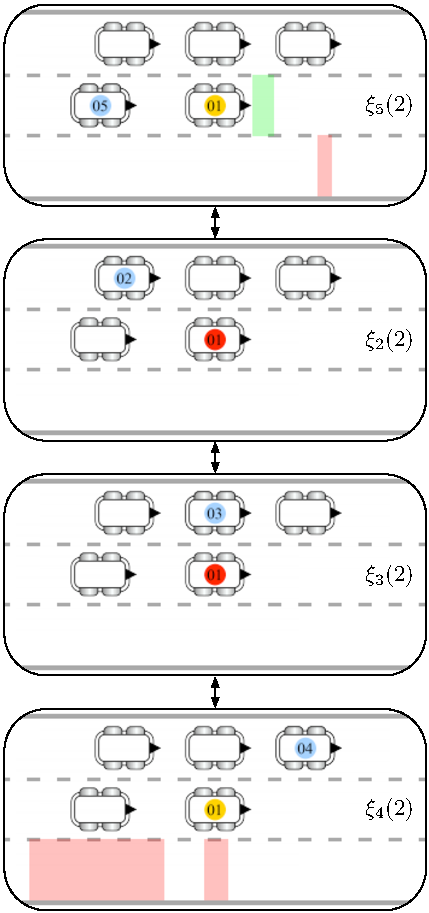
\includegraphics[width=0.22\textwidth,clip]{images/consensus-2.pdf}
&
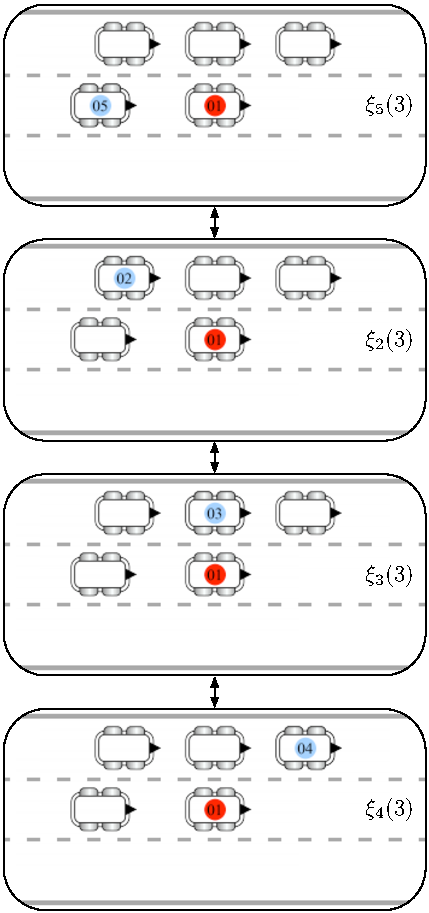
\includegraphics[width=0.22\textwidth,clip]{images/consensus-3.pdf}
\end{tabular}
\caption{Misbehavior of car~$1$ is detected by the set--valued consensus algorithm, although no single local monitor was initially able to do it.}
\label{fig:faulty-centr-consensus2}
\end{figure*}
%%

\AFnewpage
